\section{Machine Learning}

\subsection{Definition}


Machine Learning, often abbreviated as ML, is a subset of artificial intelligence (AI) that focuses on the development of computer algorithms that improve automatically through experience and by the use of data. In simpler terms, machine learning enables computers to learn from data and make decisions or predictions without being explicitly programmed to do so \cite{datacamp:ml}.

At its core, machine learning is all about creating and implementing algorithms that facilitate these decisions and predictions. These algorithms are designed to improve their performance over time, becoming more accurate and effective as they process more data.

In traditional programming, a computer follows a set of predefined instructions to perform a task. However, in machine learning, the computer is given a set of examples (data) and a task to perform, but it's up to the computer to figure out how to accomplish the task based on the examples it's given.

For instance, if we want a computer to recognize images of cats, we don't provide it with specific instructions on what a cat looks like. Instead, we give it thousands of images of cats and let the machine learning algorithm figure out the common patterns and features that define a cat. Over time, as the algorithm processes more images, it gets better at recognizing cats, even when presented with images it has never seen before.

This ability to learn from data and improve over time makes machine learning incredibly powerful and versatile. It's the driving force behind many of the technological advancements we see today, from voice assistants and recommendation systems to self-driving cars and predictive analytics.

\subsection{Relationships to other fields}

Artificial Intelligence (AI) encompasses the field of computer science dedicated to creating systems capable of emulating human-like intelligence, problem-solving, and decision-making. Machine Learning (ML) is a subset of AI focused on enabling computers to learn from data without being explicitly programmed. Within ML, Deep Learning stands out as a subfield that employs neural networks with multiple layers to learn complex representations of data, particularly effective in tasks like image and speech recognition. ML and Deep Learning are integral components of AI, providing the framework for developing intelligent systems capable of learning, reasoning, and adapting to new information, thereby advancing the capabilities of AI across various domains.

\begin{figure}[htpb]
    \centering
    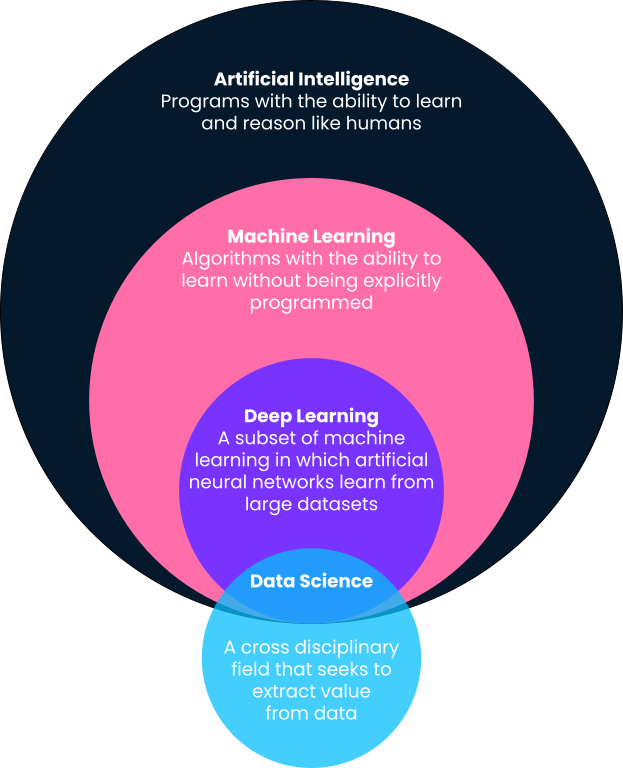
\includegraphics[width=\textwidth,height=6cm,keepaspectratio=true]{ml.png}
    \caption{
        \it{Machine learning as subfield of AI \cite{datacamp:ml}.}
    }
\end{figure}

\subsection{Types of Machine Learning}

Machine Learning can be broadly categorized into several types based on the learning approach, the availability of labeled data, and the feedback mechanism. The main types of machine learning are:

\begin{figure}[htpb]
    \centering
    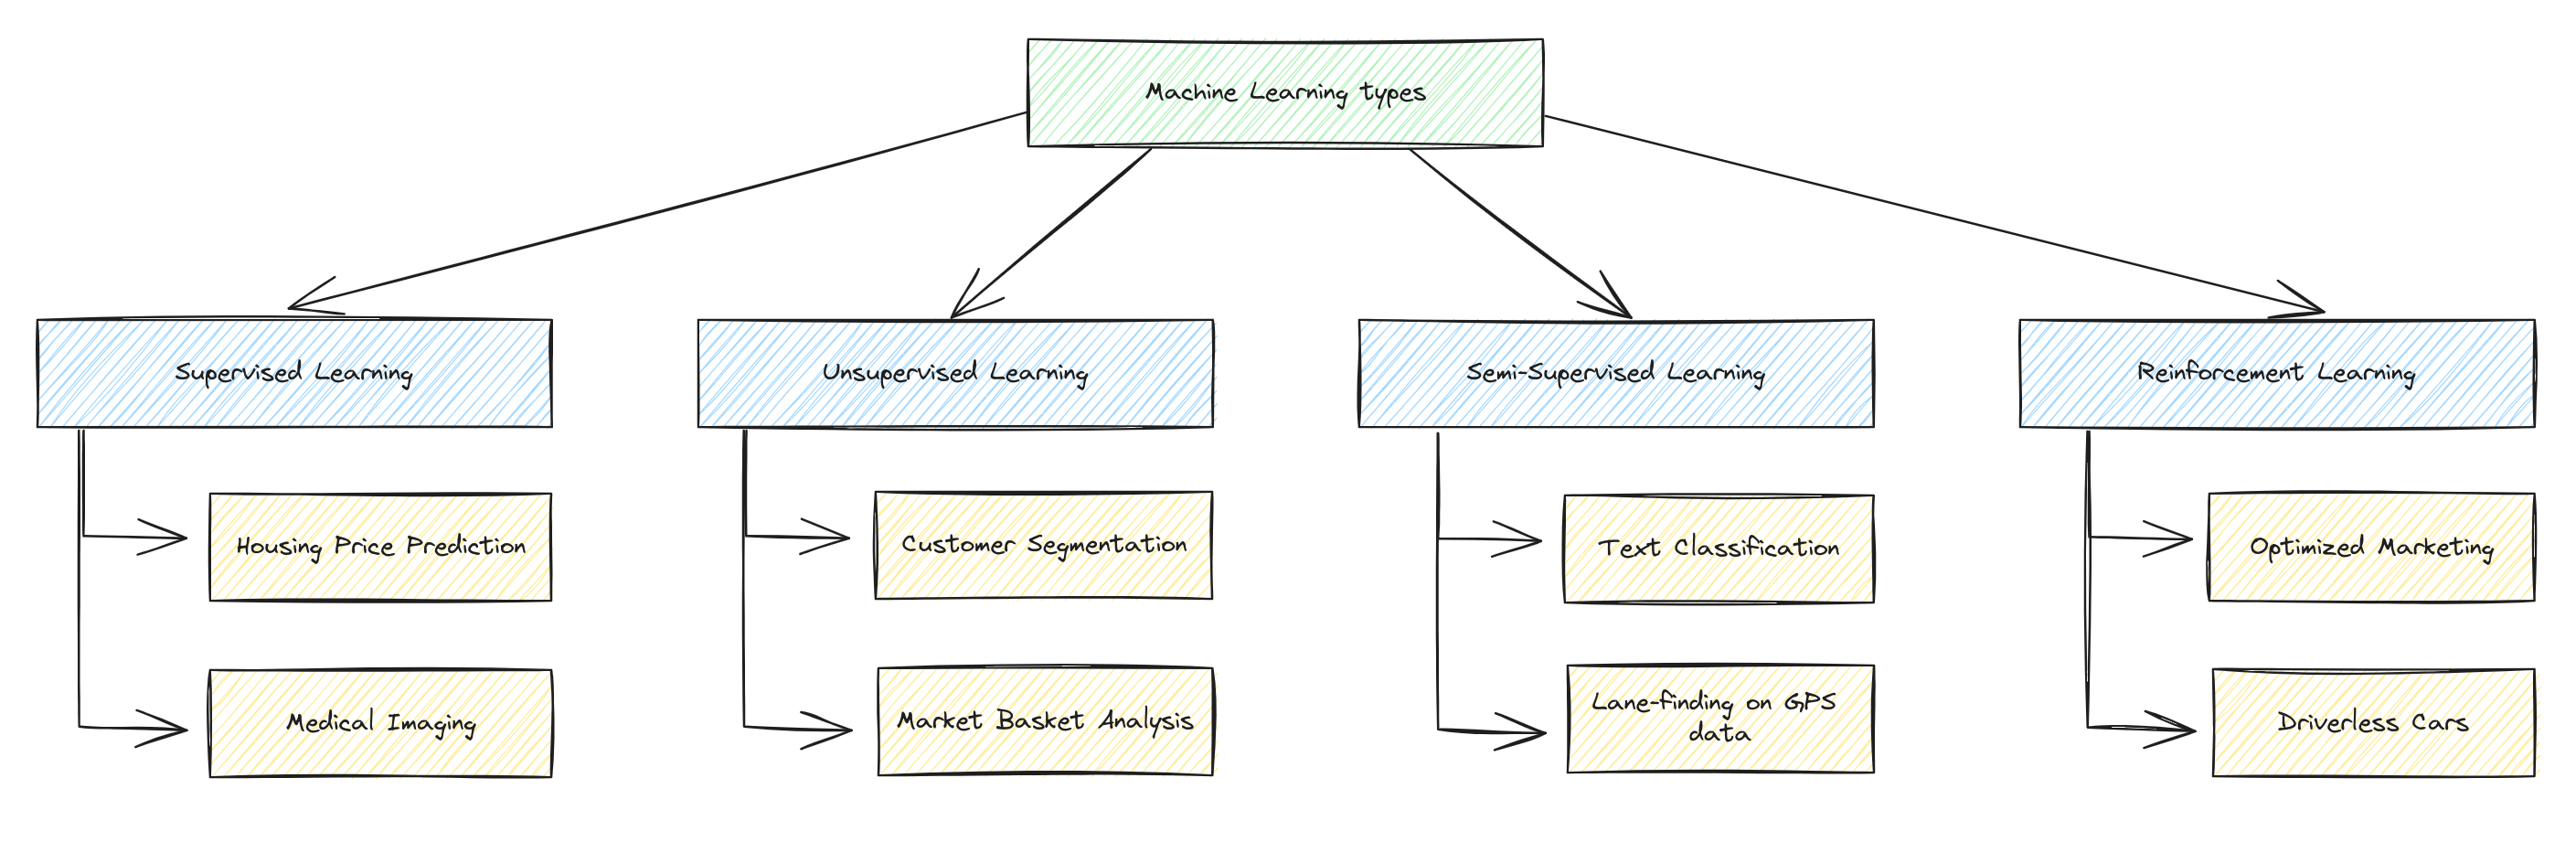
\includegraphics[width=\textwidth,height=6cm,keepaspectratio=true]{ml-types.png}
    \caption{
        \it{Types of machine Learning.}
    }
\end{figure}

\subsubsection*{Supervised Learning}
Supervised machine learning learns patterns and relationships between input and output data. It is defined by its use of labeled data. A labeled data is a dataset that contains a lot of examples of Features and Target. Supervised learning uses algorithms that learn the relationship of Features and Target from the dataset. This process is referred to as Training or Fitting \cite{datacampsupervised}.


\subsubsection*{Unsupervised Learning:}

Unsupervised learning, also known as unsupervised machine learning, uses machine learning algorithms to analyze and cluster unlabeled data sets. These algorithms discover hidden patterns or data groupings without the need for human intervention. Unsupervised learning models are utilized for three main tasks—clustering, association, and dimensionality reduction \cite{ibmunsupervised}.

\subsubsection*{Semi-Supervised Learning:}

Semi-supervised learning is a relatively new and less popular type of machine learning that, during training, blends a sizable amount of unlabeled data with a small amount of labeled data. Semi-supervised learning is between supervised learning (with labeled training data) and unsupervised learning (unlabeled training data).

Semi-supervised learning offers a lot of real-world applications. There is a dearth of labeled data in many fields. Because they involve human annotators, specialized equipment, or expensive, time-consuming studies, the labels (target variable) could be challenging to get \cite{datacampsupervised}.


\subsubsection*{Reinforcement Learning:}

Reinforcement learning (RL) is a machine learning technique that trains software to make decisions to achieve the most optimal results. It mimics the trial-and-error learning process that humans use to achieve their goals \cite{awsrl}.

\subsection{Limitations of Machine Learning: Challenges and Considerations}

Although machine learning is a powerful technique for extracting knowledge from data, it also has certain limitations that are important to consider:

\begin{itemize}
    \item{\textbf{Data dependency:} Machine learning heavily relies on the quality and quantity of training data. If the data is poorly labeled or unrepresentative, it can lead to errors in predictions.}
    \item{\textbf{Overfitting:} When the model is too complex compared to the training data, it can overfit and not generalize well to test data. This can also result in poor performance for new data.}
    \item{\textbf{Explainability:} Machine learning models can be very complex and difficult to understand. It can be challenging to understand how the model makes decisions and to explain these decisions to users.}
    \item{\textbf{Biased data:} Training data can be biased due to factors such as data selection, human biases, or measurement errors. This can lead to biased predictions for test data.}
    \item{\textbf{Lack of diversity:} Machine learning models may lack diversity in the types of data they can handle. For example, machine learning models may struggle to process unstructured data such as images, sounds, and texts.}
    \item{\textbf{Computational cost:} Machine learning algorithms may require high computational power and significant storage resources to process large amounts of data. This can be costly and time-consuming to train and implement models.}
\end{itemize}